\newpage

En el ejercicio dos se introdujeron dos familias nuevas: \textbf{Random} y \textbf{Gimnasios por grupo} que fueron explicadas apropiadamente. Como la idea es estudiar en promedio que sucede con las distancias al crecer la cantidad de elementos total del mapa (pokeparadas + gimnasios), las experimentaciones de este test se centrarán en tratar de mejorar esas distancias mediante las heurísticas introducidas en este punto ($2-opt$ y $Swap$).\\\\

Para realizar los tests se tomaron dos rangos de tamaños:
\begin{enumerate}
\item Rango 1: 5 a 15 elementos (pokeparadas + gimnasios)
\item Rango 2: 70 a 470 en intervalos de 50 elementos.
\end{enumerate}

Para el Rango 1 se tomó cinco veces el total de elementos como cantidad de instancias aleatorias por cada tamaño y para el Rango 2 se tomó un 10\% del total de elementos como cantidad de instancias aleatorias.

Se realizan las busquedas locales promediando los tiempos y distancias para todas las instancias de cada tamaño. Y se obtienen los porcentajes de mejora relativos a cada tamaño con respecto al promedio de las distancias del algoritmo goloso.
 
Para las primeras 16 instancias, se obtiene el promedio de distancias del algoritmo exacto y se calcula el error relativo en base a los promedios de las distancias obtenidas por el algoritmo goloso y las búsquedas locales.

La idea inicial del Rango 1 era poder comparar contra el backtracking las distancias obtenidas por el algoritmo goloso y las búsquedas locales, pero para instancias de 17 elementos en adelante el algoritmo demoraba demasiado tiempo y se decidió recortar hasta 16 elementos. Por cuestiones de tiempo los rangos quedaron como inicialmente se planearon.\\

\subsubsection*{Random}

Comenzando con el Rango 1 puede verse en los siguientes gráficos las mejoras realizadas por las búsquedas locales con respecto al algoritmo goloso. En promedio para cada tamaño $2-opt$ logra entre un 3\% y un 4\% de mejora más que $Swap$. Las mejoras se observan entre un 20\% y un 27\% para la mayoría de los casos.
\\\\

\begin{figure}[h] 
 \centering
  \subfloat[Distancias]{
    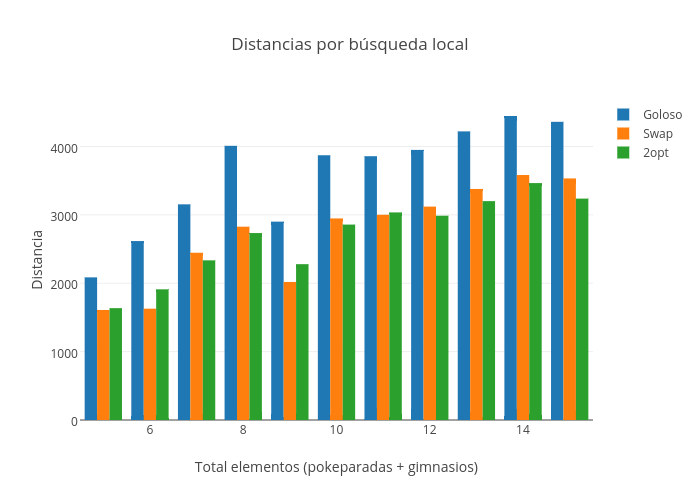
\includegraphics[width=0.45\textwidth]{./EJ3/distanciasLocales20M.png}}
       \label{fig:randomDist1}
  \subfloat[Porcentaje de mejora]{
    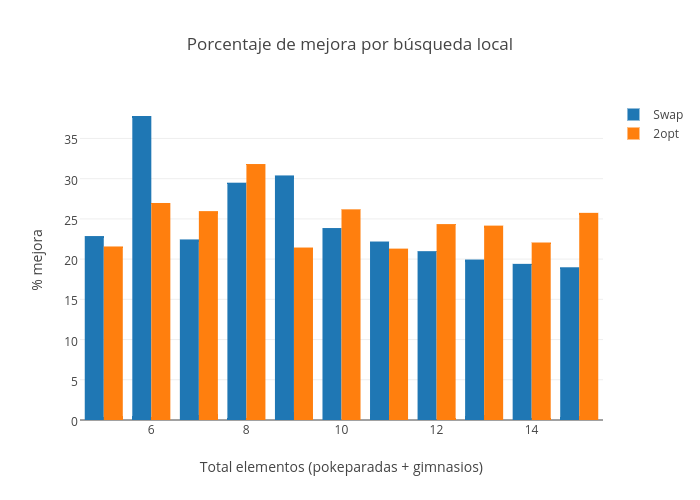
\includegraphics[width=0.45\textwidth]{./EJ3/mejoraLocales20M.png}}
    \label{fig:randomMejora1}
\end{figure}

   \vspace*{0.3cm} \vspace*{0.3cm}
  \begin{center}
	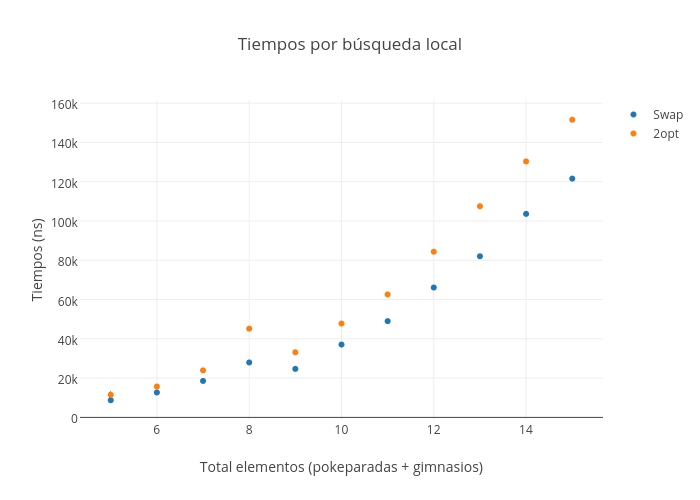
\includegraphics[scale=0.50]{./EJ3/tiemposLocales20M.png}
	\label{fig:randomTiempos1}	
	\\{\textit{Tiempos}}
  \end{center}
  \vspace*{0.3cm} 

En relación a los tiempos $Swap$ insume aproximadamente un entre un 15\% y un 20\% menos de tiempo. Esto no es considerable como para no tomar las mejoras realizadas por $2-opt$ como un buen resultado en relación calidad-performance. 
\\\\
\begin{figure}[h] 
 \centering
  \subfloat[Distancias]{
    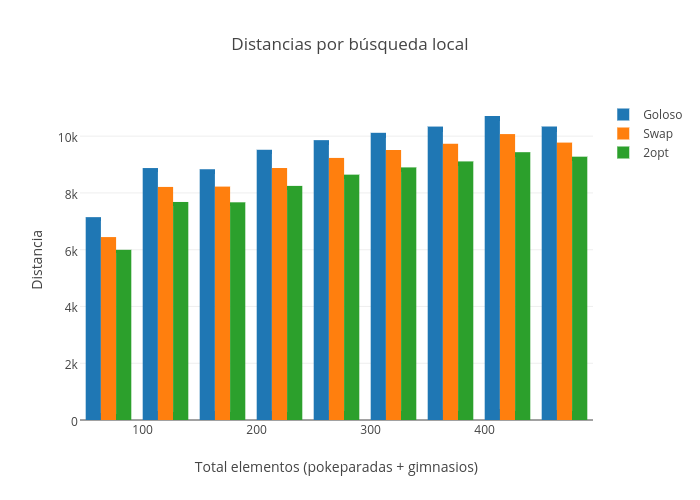
\includegraphics[width=0.45\textwidth]{./EJ3/distanciasLocales470.png}}
       \label{fig:randomDist2}
  \subfloat[Porcentaje de mejora]{
    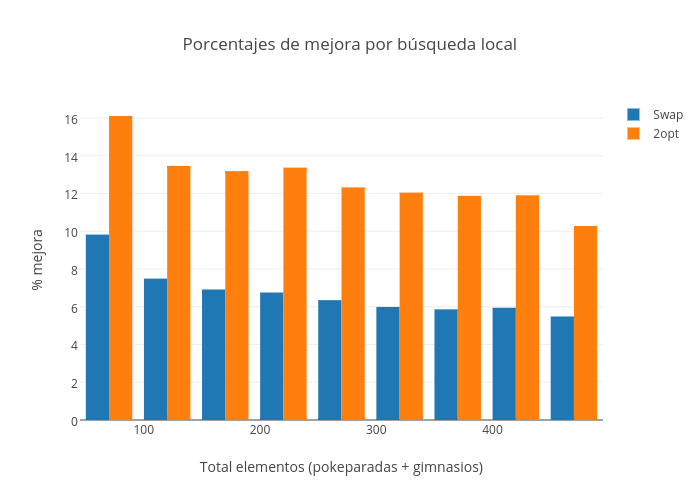
\includegraphics[width=0.45\textwidth]{./EJ3/mejoraLocales470.png}}
    \label{fig:randomMejora2}
    \end{figure}
 
   \vspace*{0.3cm} \vspace*{0.3cm}
  \begin{center}
	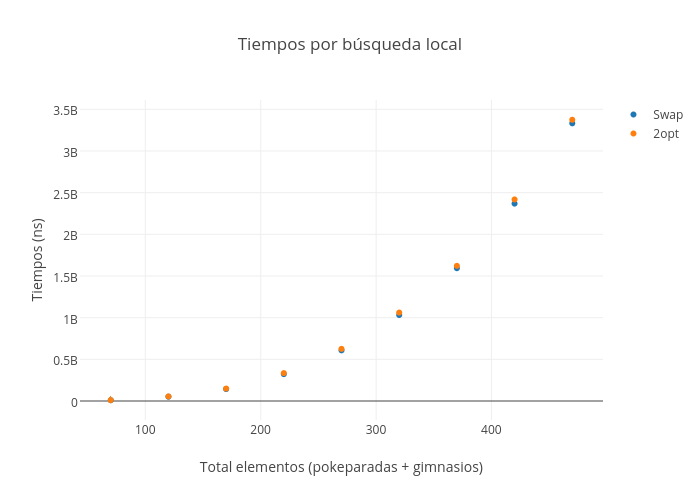
\includegraphics[scale=0.50]{./EJ3/tiemposLocales470.png}
	\label{fig:randomTiempos2}	
	\\{\textit{Tiempos}}
  \end{center}
  \vspace*{0.3cm} 

Para el Rango 2, podemos observar que a medida que el tamaño crece se observa una ligera tendencia de disminución en la mejora realizada por las búsquedas locales. Esto puede deberse al hecho de que cuanto más grande es la instancia más local se vuelve la solución realizada por el goloso y así mismo la búsqueda local solo llega a mínimos locales. Se observa igualmente un buen desempeño de la búsqueda local $2-opt$ pero con mejoras entre un 12\% y un 14\% en comparación al Rango 1. A su vez como se mencionó, para instancias mayores este porcentaje disminuye llegando a estar incluso por debajo del 12\%
\\\\
 
\newpage
\subsubsection*{Gimnasios por grupos}

Como ya sabemos, esta familia intenta organizar los gimnasios en grupos de hasta cuatro poderes distintos. Veamos que sucede al incrementar la cantidad de elementos en el mapa.

\begin{figure}[h] 
 \centering
  \subfloat[Distancias]{
    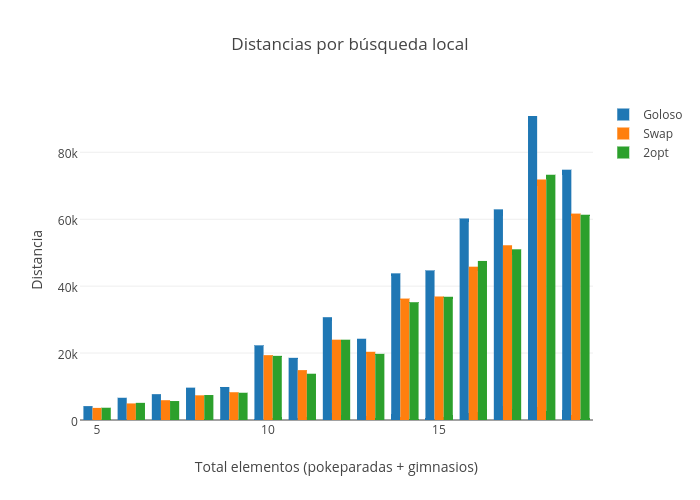
\includegraphics[width=0.45\textwidth]{./EJ3/distanciasLocales20cuadM.png}}
       \label{fig:gruposDist1}
  \subfloat[Porcentaje de mejora]{
    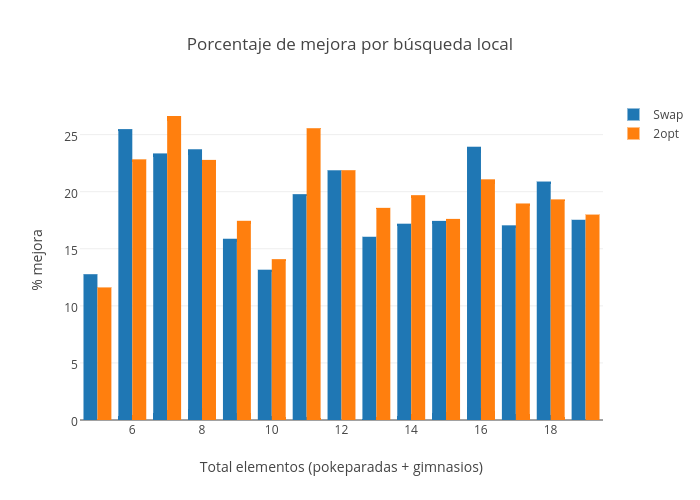
\includegraphics[width=0.45\textwidth]{./EJ3/mejoraLocales20cuadM.png}}
    \label{fig:gruposMejora1}
    \end{figure}
 
   \vspace*{0.3cm} \vspace*{0.3cm}
  \begin{center}
	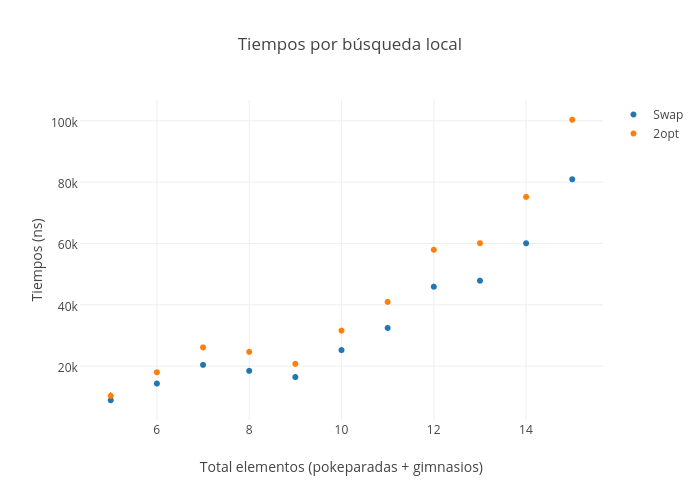
\includegraphics[scale=0.50]{./EJ3/tiemposLocales20cuadM.png}
	\label{fig:gruposTiempos1}	
	\\{\textit{Tiempos}}
  \end{center}
  \vspace*{0.3cm} 

Podemos observar en el Rango 1 como a medida que las instancias crecen en tamaño aumenta considerablemente la distancia del algoritmo goloso y las mejoras realizadas por ambas búsquedas locales son muy parecidas estando ambas por encima del 15\% en casi todos los casos. Para instancias pequeñas se hacer particularmente difícil decidir que búsqueda local es la ganadora. 
\\\\

En relación a los tiempos se observa que $Swap$ se encuentra entre un 15\% y un 20\% por debajo de $2-opt$. En relación a las mejoras obtenidas es sugerente que $Swap$ parece una buena opción para casos particularemente pequeños en relación calidad-performance.
\\\\

\begin{figure}[h] 
 \centering
  \subfloat[Distancias]{
    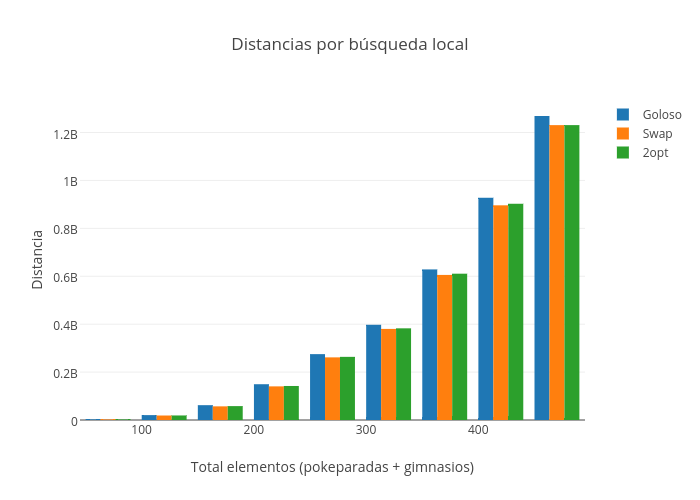
\includegraphics[width=0.45\textwidth]{./EJ3/distanciasLocales470cuad.png}}
       \label{fig:gruposDist2}
  \subfloat[Porcentaje de mejora]{
    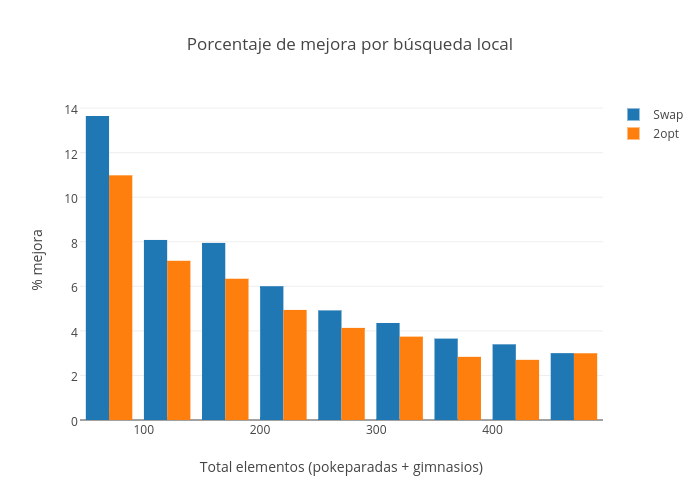
\includegraphics[width=0.45\textwidth]{./EJ3/mejoraLocales470cuad.png}}
    \label{fig:gruposMejora2}
    \end{figure}
 
   \vspace*{0.3cm} \vspace*{0.3cm}
  \begin{center}
	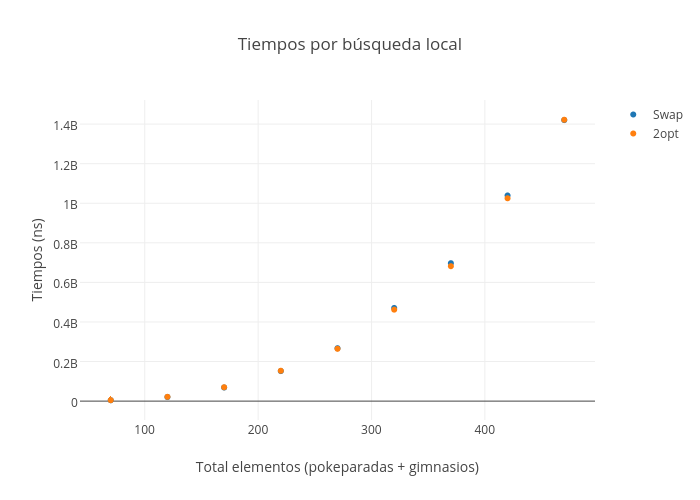
\includegraphics[scale=0.50]{./EJ3/tiemposLocales470cuad.png}
	\label{fig:gruposTiempos2}	
	\\{\textit{Tiempos}}
  \end{center}
  \vspace*{0.3cm} 
 
Para el Rango 2 se sigue observando un incremento extremadamente alto en las distancias obtenidas por el goloso. Y a su vez las mejoras realizadas por ambas búsquedas locales disminuyen conforme aumenta el tamaño. En principio se observa que no hay diferencias para instancias de 470 elementos. Debido a la discretización utilizada, este patron podría repetirse incluso a partir de los 400 elementos.

Creemos que las distancias observadas son particularmente altas debido a como están organizados los gimnasios. Al estar las pokeparadas distribuidas por todo el mapa y los gimnasios más agrupados, el algoritmo goloso deberá recorrer enormes distancias para vencer gimnasios y volver a buscar pokeparadas en la mayoria de los casos. Además debemos recordar que el algoritmo goloso no hace particular uso de la mochila ya que su premisa es siempre vencer un gimnasio cuando sea posible.

Con respecto a la disminución en los porcentajes de mejora puede observarse lo mismo que en la familia $Random$, a medida que la instancia crece, la solución se hace cada vez más local y por lo tanto las mejoras tienden a ser mínimos locales. 

Los tiempos de ambas búsquedas locales son relativamente iguales. Teniendo en cuenta la mínima ventaja de $Swap$ en cuanto a mejoras, podríamos decir que ambas búsquedas locales funcionan bien para intancias grandes.

Será particularmente importante observar en el siguiente ejercicio cuanto puede mejorar la distancia la meta heurística que será presentada, ya que queda bastante claro que los resultados del algoritmo goloso para este tipo de familia pueden ser extramadamente malos. 
\\\\

\textbf{Algún gráfico con instancias mayores a 470 elementos para mostrar que las hipótesis se cumplen?}